%Section 3: How PET/CT overcomes those challenges (physics and technical focus).
\subsection{Technical Principles of PET/CT}

Positron Emission Tomography (PET) is a functional imaging modality that uses positron-emitting radionuclides to map metabolic activity in tissues. As standalone imaging modality it lacks of anatomic structure localization, for that it is integrated with Computed Tomography (CT). CT contribution is huge, it provides attenuation correction, electron density, and anatomical localization. This way, PET/CT provides both functional and structural data in a single imaging session and with it a valuable approach in planing and diagnosing. With the use of PET annihilation gamma rays and CT high resolution it is possible to find accurately the localization of metabolic abnormalities \cite{TG174}. By taking the best of both modalities it is ensured that all metabolic information is properly contextualized on the anatomy reducing errors on registration state compared to standalone systems \cite{TG126}.

%CT
% Resolution required?

%Physics of PET/CT
%how is this acomplished
% scanner config
%technical details
%why both

The now well established Time-of-flight (TOF) technology allows to get precise timing of gamma-ray detection to improve spatial resolution and reduce noise. As it solves the problem of measure the exact site of anihilation it enchances ignal-to-noise ratio (SNR), particularly for larger patients. \cite{Seifert2022} PET technology has advanced a lot in recent years with detection enhancement, such as the adoption of Silicon Photomultiplier Arrays (SiPM) replacing older photomultiplier tubes (PMTs) augment resolution and sensitivity \cite{SunderlandSeminar}. And with it the regulations and quality assessments ensure that metrics like Standardized Uptake Value (SUV) are reliable.\cite{TG174}.

Additionally, there is another important factor related to PET scanners, as PET imaging requires administration of radiopharmaceuticals. This administration must be performed with accuracy as any error in this step, can lead to uneven tracer distribution. The next section will explore more about the particular radiotracer [18F]FDG. Sunderland et al. demonstrated that injection infiltration occurs in less than 0.4\% of cases. Moreover, computational modeling suggests that even when infiltration occurs, its impact on dosimetry and image quality is negligible  \cite{Sunderland2023}. 


\subsection{Mechanism of [18F]FDG Uptake}


Fluorine-18 Fluorodeoxyglucose or [18F]FDG is a glucose analog labeled with the positron-emitting isotope fluorine-18. After intravenous injection, FDG is transported into cells by glucose transporters like GLUT1 and  the enzyme hexokinase adds a phosphate group (phosphorylase) to it. Since this is now a different molecule from glucose cells cannot longer proceed in the glycolysis process, and the molecule gets trapped in cells with high glucose metabolism, such as tumor cells \cite{TG174, Zheng2018}.

This characteristic of the cancer cell is what allows for PET to visualize regions of hyperglycolysis. For example, as shown in Figure \ref{fig:PuFig1}, PET images A) show regions of increased metabolic activity in the pancreatic head, in B) CT images provide anatomical context. The fused PET/CT image C) integrates these modalities, and allows for precise localization of pancreatic tumors.
Then oncogenic mutations like KRAS drive this process by upregulating GLUT1 and hexokinase-2, further amplifying glucose uptake \cite{Deng2021}. But this is not the only reason FDG accumlation can increase, this behaivior is also present in inflammation and benign conditions, such as autoimmune pancreatitis \cite{Zheng2018}. Different radiotracers may shine some light into the problems faced right now and and with them new advancements in tracer specificity and imaging protocols emerge.

\begin{figure}[H]
	\centering
	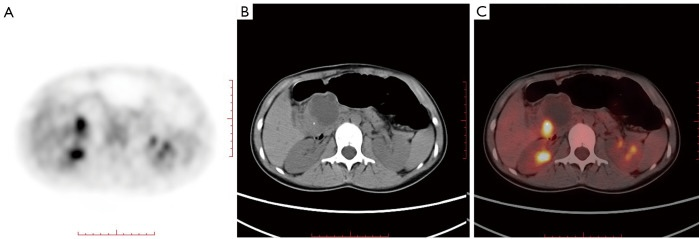
\includegraphics[width=0.9\textwidth]{assets/tcr-10-07-3560-f1.jpg}
	\caption{18F-FDG PET/CT imaging integrating metabolic and anatomical data: (A) PET image, (B) non-enhanced CT image, (C) fused PET and CT images, demonstrating pancreatic head cancer detection \cite{Pu2021}.}
	\label{fig:PuFig1}
\end{figure}
